\subsubsection{Concept 1}

The first concept is the use of a stereo vision camera to detect a suitable object to perch from.
This appreach has been established in existing literature, such as the perching mechanisms developed by
Kominami et al. \cite{kominami_detection_2023} and von Frankenberg et al. \cite{von_frankenberg_detection_2020}.

Dual cameras would be used to calculate a depth map, from which the location and orientation of a perchable object, like 
a tree branch or power line, can then be detected. 

A proof of concept image processing pipeline for this method was developed and tested in Python.
It is based on the method proposed by Kominami et al., in which a Hough transform detects the two
sides of a possible perch, and the depth profile along a path perpendicular to the two lines is 
used to verify that the detected object is a suitable perch \cite{kominami_detection_2023}.
Modifications to the exact detection method and criteria are made to address the difference 
in perch types between Kominami et al. and this work; while Kominami at al. are focusing 
on detecting thin vertical boards, this mechanism needs to itentify cylindrical shapes.

The steps in the pipeline proposed are as follows:

\begin{enumerate}
    \item Stereo image aquisition:
        Images from two cameras are aquired, rectified, and processed to produce a disparity image.
    \item The disparity image is projected to a point cloud in the left cameras cordinate frame,
        then converted to a depth image.
    \item Missing data in the depth image is inpainted using the Fast Marching Method developed by
        Telea \cite{telea_image_2004}.
    \item The depth image is filtered using guided filtering \cite{he_guided_2013}, 
        with the left cameras refified grayscale image as a guide. This is intended to
        remove noise while preserving sharp details of object borders.
    \item A Canny edge detector is applied to the grayscale image of the left camera.
    \item A probabilistic Hough transform is applied to identify line segments in the image.
    \item Parallel pairs are identified from the set of line segments.
    \item For each parallel pair, a perpendicular line is found and the depth profile along 
        that line is sampled.
\end{enumerate}


\paragraph{Budget}

\begin{table}[ht]
    \centering
    \caption{Estimated budget for the stereo camera sensing design.}
    \label{tab:stereo}


    \begin{spreadtab}{{tabular}{|c|c|c|c||c|}}
        \hline
        @Item                       & @Supplier                                                                                                         & @Unit Cost (USD) & @Quantity & @Total Cost (USD) \\
        \hline
        @SMA Wire                   & @\href{https://www.kelloggsresearchlabs.com/product/round-wire/}{Kelloggs Research Labs}                          & 15.99 & 1 & [-1,0] * [-2,0] tag(start) \\
        @Mechanical Materials and Fabrication & @-                                                                                                      &     0 & 1 & [-1,0] * [-2,0] tag(pretax)\\
        @Tax                        & @- & sum(cell(start):cell(pretax)) * 0.07 & 1 & [-1,0] * [-2,0] tag(posttax) \\
        @Misc. Spares               & @- & sum(cell(start):cell(posttax)) * 0.2 & 1 & [-1,0] * [-2,0] tag(end) \\
        \hline
        \multicolumn{4}{|c||}{@Total} & sum(cell(start):cell(end)) \\
        \hline
    \end{spreadtab}
\end{table}


\paragraph{Evaluation}

The main downside of this method is that it is the highest cost and weight of all the options, due to 
the requirement of two cameras. Aquiring quality depth images with low processing time is another challenge.
The disparity maps produced by block matching are noisy and have many patches of missing data. Inpainting
and guided filtering help with this, but there remain a large number of artifacts in the depth data
that interfere with identifying suitable objects for perching.

Figure \ref{fig:c1:depth_profiles} shows images from the proof of concept pipeline, obtained from 
processing figure \ref{fig:c1:testimg}. All image processing functions used are implemented by OpenCV.

\begin{figure}[H]
    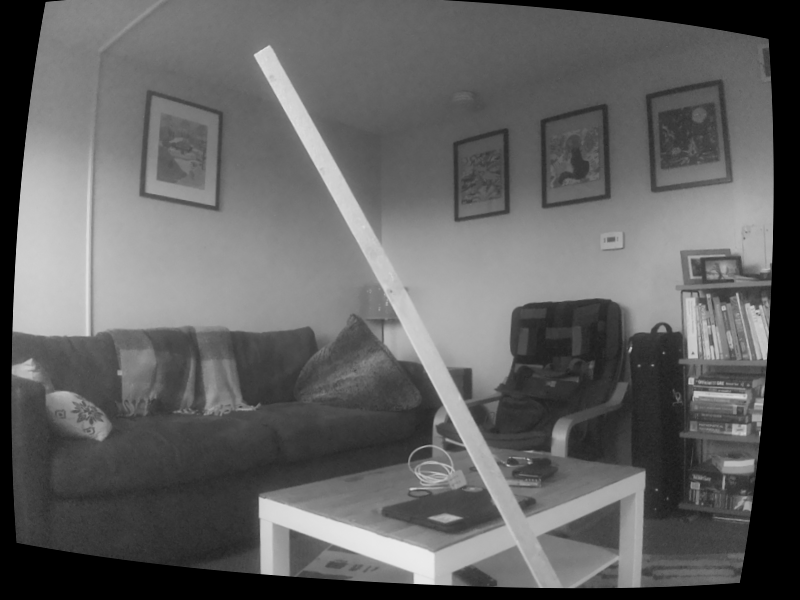
\includegraphics[width=0.5\textwidth]{sections/sensor_concepts/left.png}
    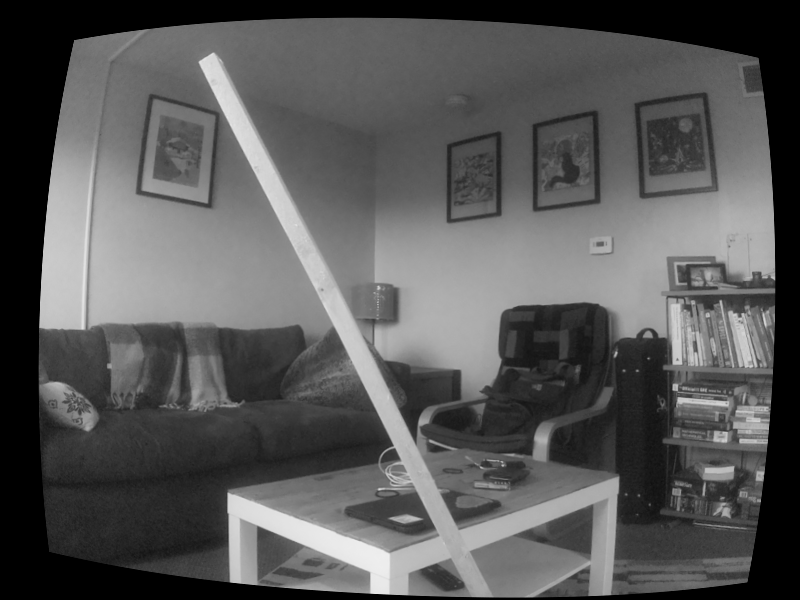
\includegraphics[width=0.5\textwidth]{sections/sensor_concepts/right.png}
    \caption{Captures from left and right cameras used as input in this proof of concept.
    In the center of the frame is a rectangular wooden plank, used as a target perch to detect.
    }
    \label{fig:c1:testimg}
\end{figure}

\begin{figure}[H]
    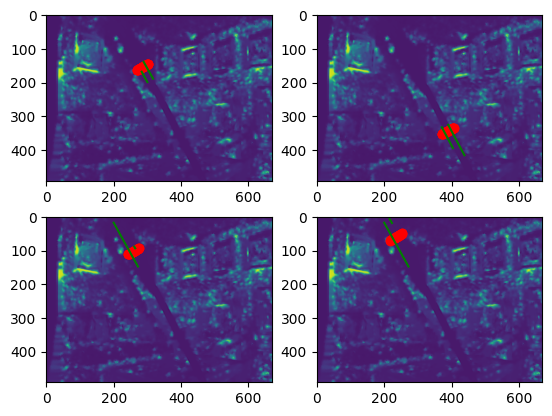
\includegraphics[width=0.5\textwidth]{sections/sensor_concepts/test_perch_lines.png}
    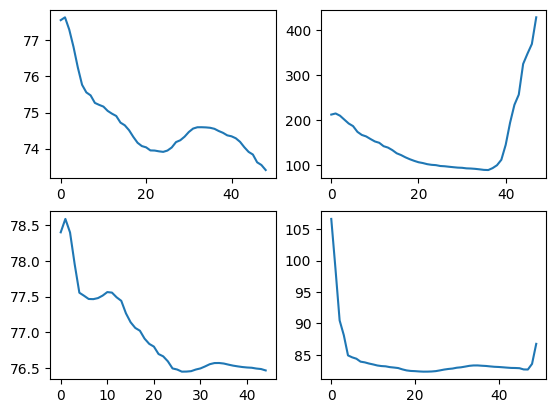
\includegraphics[width=0.5\textwidth]{sections/sensor_concepts/test_perch_profiles.png}
    \caption{Sample images from the proof of concept pipeline. The left images show 4 pairs of 
    parallel lines identified in figure \ref{fig:c1:testimg} (the parallel lines are drawn in green),
    as well as the perpendicular path traced for each pair of lines (the thicker line drawn in red).
    The right images show the depth profiles along the perpendicular path for each pair of lines.
    Note the high distortion around the edges of the target perch, particularly near the top end.
    The ideal depth profile for this perch would be a box function, where the high level indicates the
    distance to the perch and the width of the box corresponds to the width of the perch.
    }
    \label{fig:c1:depth_profiles}
\end{figure}

The depth images produces here have large amounts of noise and error, which interferes with identification of
suitable perches based on depth profiles. The errors in the depth image may be due to poor stereo calibration.
They may also be due to poor inpainting of missing regions. An attempt was made to implement the guided inpainting 
described by Gong et al. \cite{gong_guided_2013}, however so far implementing this algorithm has been unsuccesfull.


